\begin{frontpage}

%\begin{figure}[ht!]
%\noindent \includegraphics[scale=1]{1-Preamble/1-Front/couverture_these_lilianbesson1.eps}
%\end{figure}

% \includepdf[pages={1}]{1-Preamble/1-Front/couverture_these_lilianbesson2.pdf}
\includepdf[pages={1}]{1-Preamble/1-Front/couverture_these_lilianbesson3.pdf}
% \includepdf[pages={1}]{1-Preamble/1-Front/couverture_these_lilianbesson4.pdf}
%\begin{center}

%\end{center}

%\includegraphics [width=\linewidth]{f1-Preamble/1-Front/Couverture_these}
%\iffalse
%	% Std 1 inch margin for the 1st page
%	\newgeometry{margin=1in}
%
%	% Set path for images
%	\graphicspath{{1-Preamble/1-Front/Images/}}
%
%	\begin{center}
%
%		\begin{figure}[!htb]
%			
\includegraphics[height=2.5cm]{CS.eps}
%			\hfill
%			
\includegraphics[height=2.5cm]{mathstic.eps}
%		\end{figure}
%
%		\textFF{\large N° d'ordre : 2017-XX-TH}
%		\hfill
%		\textFF{\large Année 2019}
%
%		\vspace{1cm}
%		\textbf{\textFF{\huge THÈSE DE DOCTORAT}}
%
%		\vspace{0.7cm}
%		\textbf{\textFF{\large Domaine : STIC}}
%
%		\vspace{-0.1cm}
%		\textbf{\textFF{\large Spécialité : Télécommunications}}
%
%		\vspace{0.0cm}
%		\textbf{\textFF{\LARGE \'Ecole Doctorale MATHSTIC}}
%
%		\vspace{0.7cm}
%		\textit{\textbf{\textFF{\large présentée par}}}
%
%		\vspace{0.3cm}
%		\textbf{\textFF{\Huge Lilian Besson}}
%
%		\vspace{1.0cm}
%		\textbf{\textFF{\large Sujet :}}
%
%		\vspace{0.5cm}
%		\hrule
%		\vspace{0.1cm}
%		{\fontsize{19}{23}\selectfont \textbf{\textFF{Mon titre de ouf}}}
%		\vspace{0.4cm}
%		\hrule
%	\end{center}
%
%	\vfill
%	%\left
%	\textFF{\large Soutenue à Rennes le xx octobre 2019 devant le jury composé de :}
%
%	\begin{tabbing}
%		\textit{\textFF{Dir. de Thèse :}} \hspace{1cm} \= \textbf{\textFF{Christophe Moy}} \hspace{2cm} \= \textFF{Professeur, Université de Rennes 1} \\
%		\textit{\textFF{Encadrants :}} \> \textbf{\textFF{Emilie Kaufmann}} \> \textFF{Professeur, Université de Rennes 1}\\
%		\textit{\textFF{Rapporteurs :}} \> \textbf{\textFF{Antoine DUPONT}} \> \textFF{Professeur, ABCDE, Nouvelle-Zélande}\\
%										\> \textbf{\textFF{Alexandre DUPOND}} \> \textFF{Maître de Conférence, FGHIJ, Papouasie}\\
%		\textit{\textFF{Examinateurs :}}\> \textbf{\textFF{Alexandra DURAND}} \> \textFF{Professeur, KLM, Pays-Bas}\\
%										\> \textbf{\textFF{Prénom SUPERNOM}} \> \textFF{Docteur, Super Labo, SPLand}
%	\end{tabbing}
%
%	% Set classical geometry for the rest of the thesis
%	\restoregeometry
%\fi
\end{frontpage}

